\subsection{Syntax Level}
\label{syntax}
The syntax level is the lowest abstraction level in our taxonomy. This level includes the most basic programming functionality like syntax and code compilations. This level does not require the \cct{} suggested code to successfully perform the task but to suggest code without any obvious errors like syntax errors.
For example, consider a task of perform a sorting operation on a list of numbers. To satisfy this level of abstraction, \cct{} should suggest code that is syntactically correct without any compilation errors and the code is not required to perform the sorting operation correctly. 
Figure~\ref{fig:syntax} shows the example and syntax suggestions from \cct{} at this abstraction level.

\begin{figure}[hbt!]
    \centering
    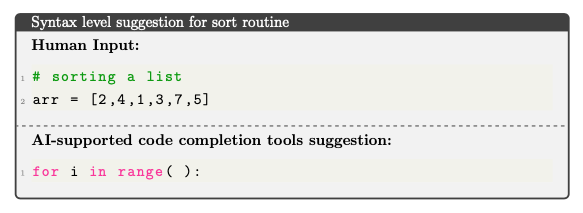
\includegraphics[width=\linewidth]{Figures/syntax.png}
    \caption{\cct{} syntax level suggestions}
    \label{fig:syntax}
\end{figure}

The goal of this software abstraction level in our taxonomy is for a \cct{} to be able to suggest code without any syntactical errors.
The capabilities required by \cct{} to satisfy this level of abstraction are as follows:

\begin{enumerate}
    \item Suggested code should be syntactically correct.
    \item Suggested code should not produce any errors in code compilation.
\end{enumerate}

% \begin{tcolorbox}[title=Syntax level suggestion for sort routine,boxsep=.15mm]
%     %https://tex.stackexchange.com/questions/337909/tcolorbox-tcbline-style
% \textbf{Human Input:}
% \begin{lstlisting}[language={Python}]
% # sorting a list
% arr = [2,4,1,3,7,5]
% \end{lstlisting}
% \tcbline
% \textbf{\cct{} suggestion:}
% \begin{lstlisting}[language={Python}]
% for i in range( ):
% \end{lstlisting}
% \end{tcolorbox}